% Options for packages loaded elsewhere
\PassOptionsToPackage{unicode}{hyperref}
\PassOptionsToPackage{hyphens}{url}
%
\documentclass[
]{article}
\usepackage{lmodern}
\usepackage{amssymb,amsmath}
\usepackage{ifxetex,ifluatex}
\ifnum 0\ifxetex 1\fi\ifluatex 1\fi=0 % if pdftex
  \usepackage[T1]{fontenc}
  \usepackage[utf8]{inputenc}
  \usepackage{textcomp} % provide euro and other symbols
\else % if luatex or xetex
  \usepackage{unicode-math}
  \defaultfontfeatures{Scale=MatchLowercase}
  \defaultfontfeatures[\rmfamily]{Ligatures=TeX,Scale=1}
\fi
% Use upquote if available, for straight quotes in verbatim environments
\IfFileExists{upquote.sty}{\usepackage{upquote}}{}
\IfFileExists{microtype.sty}{% use microtype if available
  \usepackage[]{microtype}
  \UseMicrotypeSet[protrusion]{basicmath} % disable protrusion for tt fonts
}{}
\makeatletter
\@ifundefined{KOMAClassName}{% if non-KOMA class
  \IfFileExists{parskip.sty}{%
    \usepackage{parskip}
  }{% else
    \setlength{\parindent}{0pt}
    \setlength{\parskip}{6pt plus 2pt minus 1pt}}
}{% if KOMA class
  \KOMAoptions{parskip=half}}
\makeatother
\usepackage{xcolor}
\IfFileExists{xurl.sty}{\usepackage{xurl}}{} % add URL line breaks if available
\IfFileExists{bookmark.sty}{\usepackage{bookmark}}{\usepackage{hyperref}}
\hypersetup{
  pdftitle={Bioinformatics},
  hidelinks,
  pdfcreator={LaTeX via pandoc}}
\urlstyle{same} % disable monospaced font for URLs
\usepackage[margin=1in]{geometry}
\usepackage{graphicx,grffile}
\makeatletter
\def\maxwidth{\ifdim\Gin@nat@width>\linewidth\linewidth\else\Gin@nat@width\fi}
\def\maxheight{\ifdim\Gin@nat@height>\textheight\textheight\else\Gin@nat@height\fi}
\makeatother
% Scale images if necessary, so that they will not overflow the page
% margins by default, and it is still possible to overwrite the defaults
% using explicit options in \includegraphics[width, height, ...]{}
\setkeys{Gin}{width=\maxwidth,height=\maxheight,keepaspectratio}
% Set default figure placement to htbp
\makeatletter
\def\fps@figure{htbp}
\makeatother
\setlength{\emergencystretch}{3em} % prevent overfull lines
\providecommand{\tightlist}{%
  \setlength{\itemsep}{0pt}\setlength{\parskip}{0pt}}
\setcounter{secnumdepth}{-\maxdimen} % remove section numbering
\usepackage{booktabs}
\usepackage{longtable}
\usepackage{array}
\usepackage{multirow}
\usepackage{wrapfig}
\usepackage{float}
\usepackage{colortbl}
\usepackage{pdflscape}
\usepackage{tabu}
\usepackage{threeparttable}
\usepackage{threeparttablex}
\usepackage[normalem]{ulem}
\usepackage{makecell}
\usepackage{xcolor}

\title{Bioinformatics}
\author{}
\date{\vspace{-2.5em}}

\begin{document}
\maketitle

\hypertarget{disease-description-hepatoma}{%
\subsection{Disease Description:
Hepatoma}\label{disease-description-hepatoma}}

Novikoff hepatoma mitochondria were studied with regard to their
functional and structural organiza-tion. The activities of cytochrome
oxidase and malate dehydrogenase in mitochondria purified on su-crose
gradients were similar in organelles derived from normal liver and
hepatoma tissue. However, the activities of reduced nicotinamide adenine
dinucleotide oxidase and succinate oxidase in hepato-ma mitochondria
were reduced to only 10 and 35\%, respectively, of the activities in
liver mitochondria. Also, monoamine oxidase and rotenone-insensitive
reduced nicotinamide adenine dinucleotide-cytochrome c reductase
(enzymes localized in the outer mitochondrial membrane) have
significantly reduced activities in hepatoma mitochondria. The
structural changes in hepatoma mitochondria might be correlated with
differences in the banding patterns of liver and hepatoma mitochondria
in sucrose gradients. While liver mitochondria banded sharply at a
density of 1.187 g/ml, as evidenced by marker enzyme activity and
protein assay, hepatoma mitochondria were heterogeneous, banding over a
den-sity range of 1.144 to 1.161 g/ml. The addition of 1\% bovine serum
albumin to the isolation medium increased the density of hepatoma
mitochondria in sucrose gradients to 1.171 g/ml and resulted in sharp,
homogeneous bands. This increase in density is due in part to protein
binding, as evidenced by bovine serum albumin-14C-binding experiments.
In addition, hepatoma mitochondria were shown to be heterogeneous by
their separation into three density classes on discontinuous bovine
serum al-bumin gradients.

\hypertarget{seed-genes}{%
\subsection{Seed genes}\label{seed-genes}}

To collect the set of seed genes we started by filtering the ``Curated
gene-disease associations'' da-taset from DisGeNet in order to find all
the genes associated with hepatoma, making sure they were all human
genes. Subsequently, we used the REST API of HGNC to fetch the status
(approved or not) of each seed gene. All the 110 genes collected from
DisGeNet resulted approved on HGNC, so we parsed the Uniprot dataset and
collected the information requested in 1.1.b. We found that only 80 of
the 110 seed genes resulted officially reviewed on Uniprot. All the data
collected has been stored in a .tsv file.

\hypertarget{table-visualization}{%
\subsubsection{Table visualization}\label{table-visualization}}

\begin{table}[H]
\centering
\begin{tabular}[t]{r|l|l|l|l}
\hline
geneId & geneSymbol & uniprotAC & proteinName & notes\\
\hline
174 & AFP & P02771 & Alpha-fetoprotein & \\
\hline
212 & ALAS2 & P22557 & 5-aminolevulinate synthase & -\\
\hline
337 & APOA4 & P06727 & Apolipoprotein A-IV & -\\
\hline
344 & APOC2 & P02655 & Apolipoprotein C-II & -\\
\hline
355 & FAS & P25445 & Tumor necrosis factor receptor superfamily member 6 & -\\
\hline
538 & ATP7A & Q04656 & Copper-transporting ATPase 1 & -\\
\hline
540 & ATP7B & P35670 & Copper-transporting ATPase 2 & -\\
\hline
578 & BAK1 & Q16611 & Bcl-2 homologous antagonist/killer & -\\
\hline
595 & CCND1 & P24385 & G1/S-specific cyclin-D1 & -\\
\hline
596 & BCL2 & P10415 & Apoptosis regulator Bcl-2 & -\\
\hline
598 & BCL2L1 & Q07817 & Bcl-2-like protein 1 & -\\
\hline
967 & CD63 & P08962 & CD63 antigen & -\\
\hline
999 & CDH1 & P12830 & Cadherin-1 & -\\
\hline
1317 & SLC31A1 & O15431 & High affinity copper uptake protein 1 & -\\
\hline
1356 & CP & P00450 & Ceruloplasmin & -\\
\hline
1499 & CTNNB1 & P35222 & Catenin beta-1 & -\\
\hline
1544 & CYP1A2 & P05177 & Cytochrome P450 1A2 & -\\
\hline
1571 & CYP2E1 & P05181 & Cytochrome P450 2E1 & -\\
\hline
2026 & ENO2 & P09104 & Gamma-enolase & -\\
\hline
2161 & F12 & P00748 & Coagulation factor XII & -\\
\hline
2305 & FOXM1 & Q08050 & Forkhead box protein M1 & -\\
\hline
2705 & GJB1 & P08034 & Gap junction beta-1 protein & -\\
\hline
2752 & GLUL & P15104 & Glutamine synthetase & -\\
\hline
2922 & GRP & P07492 & Gastrin-releasing peptide & -\\
\hline
2950 & GSTP1 & P09211 & Glutathione S-transferase P & -\\
\hline
3082 & HGF & P14210 & Hepatocyte growth factor & -\\
\hline
3265 & HRAS & P01112 & GTPase HRas & -\\
\hline
3569 & IL6 & P05231 & Interleukin-6 & -\\
\hline
3717 & JAK2 & O60674 & Tyrosine-protein kinase JAK2 & -\\
\hline
3791 & KDR & P35968 & Vascular endothelial growth factor receptor 2 & -\\
\hline
3845 & KRAS & P01116 & GTPase KRas & -\\
\hline
4233 & MET & P08581 & Hepatocyte growth factor receptor & -\\
\hline
4240 & MFGE8 & Q08431 & Lactadherin & -\\
\hline
4283 & CXCL9 & Q07325 & C-X-C motif chemokine 9 & -\\
\hline
4313 & MMP2 & P08253 & 72 kDa type IV collagenase & -\\
\hline
4609 & MYC & P01106 & Myc proto-oncogene protein & -\\
\hline
5052 & PRDX1 & Q06830 & Peroxiredoxin-1 & -\\
\hline
5371 & PML & P29590 & Protein PML & -\\
\hline
5471 & PPAT & Q06203 & Amidophosphoribosyltransferase & -\\
\hline
5594 & MAPK1 & P28482 & Mitogen-activated protein kinase 1 & -\\
\hline
5595 & MAPK3 & P27361 & Mitogen-activated protein kinase 3 & -\\
\hline
5925 & RB1 & P06400 & Retinoblastoma-associated protein & -\\
\hline
6364 & CCL20 & P78556 & C-C motif chemokine 20 & -\\
\hline
6659 & SOX4 & Q06945 & Transcription factor SOX-4 & -\\
\hline
6696 & SPP1 & P10451 & Osteopontin & -\\
\hline
6713 & SQLE & Q14534 & Squalene monooxygenase & -\\
\hline
6774 & STAT3 & P40763 & Signal transducer and activator of transcription 3 & -\\
\hline
7010 & TEK & Q02763 & Angiopoietin-1 receptor & -\\
\hline
7039 & TGFA & P01135 & Protransforming growth factor alpha [Cleaved into: Transforming growth factor alpha & -\\
\hline
7040 & TGFB1 & P01137 & Transforming growth factor beta-1 proprotein [Cleaved into: Latency-associated peptide & -\\
\hline
7083 & TK1 & P04183 & Thymidine kinase & -\\
\hline
7124 & TNF & P01375 & Tumor necrosis factor & -\\
\hline
7157 & TP53 & P04637 & Cellular tumor antigen p53 & -\\
\hline
8517 & IKBKG & Q9Y6K9 & NF-kappa-B essential modulator & -\\
\hline
8651 & SOCS1 & O15524 & Suppressor of cytokine signaling 1 & -\\
\hline
8795 & TNFRSF10B & O14763 & Tumor necrosis factor receptor superfamily member 10B & -\\
\hline
8848 & TSC22D1 & Q15714 & TSC22 domain family protein 1 & -\\
\hline
9104 & RGN & Q15493 & Regucalcin & -\\
\hline
9970 & NR1I3 & Q14994 & Nuclear receptor subfamily 1 group I member 3 & -\\
\hline
22800 & RRAS2 & P62070 & Ras-related protein R-Ras2 & -\\
\hline
23582 & CCNDBP1 & O95273 & Cyclin-D1-binding protein 1 & -\\
\hline
27113 & BBC3 & Q9BXH1 & Bcl-2-binding component 3 & -\\
\hline
219972 & MPEG1 & Q2M385 & Macrophage-expressed gene 1 protein & -\\
\hline
283120 & H19 & - & - & Not in Uniprot.\\
\hline
406884 & MIRLET7B & - & - & Not in Uniprot.\\
\hline
406886 & MIRLET7D & - & - & Not in Uniprot.\\
\hline
406887 & MIRLET7E & - & - & Not in Uniprot.\\
\hline
406891 & MIRLET7I & - & - & Not in Uniprot.\\
\hline
406902 & MIR10A & - & - & Not in Uniprot.\\
\hline
406910 & MIR125A & - & - & Not in Uniprot.\\
\hline
406937 & MIR145 & - & - & Not in Uniprot.\\
\hline
406953 & MIR18A & - & - & Not in Uniprot.\\
\hline
406957 & MIR181C & - & - & Not in Uniprot.\\
\hline
406959 & MIR183 & - & - & Not in Uniprot.\\
\hline
406962 & MIR186 & - & - & Not in Uniprot.\\
\hline
406971 & MIR195 & - & - & Not in Uniprot.\\
\hline
406984 & MIR200B & - & - & Not in Uniprot.\\
\hline
406989 & MIR206 & - & - & Not in Uniprot.\\
\hline
406994 & MIR212 & - & - & Not in Uniprot.\\
\hline
407006 & MIR221 & - & - & Not in Uniprot.\\
\hline
407017 & MIR26B & - & - & Not in Uniprot.\\
\hline
407027 & MIR301A & - & - & Not in Uniprot.\\
\hline
407029 & MIR30A & - & - & Not in Uniprot.\\
\hline
407030 & MIR30B & - & - & Not in Uniprot.\\
\hline
407033 & MIR30D & - & - & Not in Uniprot.\\
\hline
407034 & MIR30E & - & - & Not in Uniprot.\\
\hline
407040 & MIR34A & - & - & Not in Uniprot.\\
\hline
407054 & MIR98 & - & - & Not in Uniprot.\\
\hline
407056 & MIR99B & - & - & Not in Uniprot.\\
\hline
442898 & MIR324 & - & - & Not in Uniprot.\\
\hline
442903 & MIR331 & - & - & Not in Uniprot.\\
\hline
442904 & MIR335 & - & - & Not in Uniprot.\\
\hline
442906 & MIR338 & - & - & Not in Uniprot.\\
\hline
442907 & MIR339 & - & - & Not in Uniprot.\\
\hline
442908 & MIR340 & - & - & Not in Uniprot.\\
\hline
442920 & MIR196B & - & - & Not in Uniprot.\\
\hline
494332 & MIR383 & - & - & Not in Uniprot.\\
\hline
554210 & MIR429 & - & - & Not in Uniprot.\\
\hline
574413 & MIR409 & - & - & Not in Uniprot.\\
\hline
574457 & MIR181D & - & - & Not in Uniprot.\\
\hline
574508 & MIR505 & - & - & Not in Uniprot.\\
\hline
619552 & MIR483 & - & - & Not in Uniprot.\\
\hline
664612 & MIR539 & - & - & Not in Uniprot.\\
\hline
693183 & MIR598 & - & - & Not in Uniprot.\\
\hline
693235 & MIR92B & - & - & Not in Uniprot.\\
\hline
724022 & MIR652 & - & - & Not in Uniprot.\\
\hline
768213 & MIR671 & - & - & Not in Uniprot.\\
\hline
100126297 & MIR300 & - & - & Not in Uniprot.\\
\hline
100126333 & MIR708 & - & - & Not in Uniprot.\\
\hline
100126348 & MIR760 & - & - & Not in Uniprot.\\
\hline
\end{tabular}
\end{table}

\hypertarget{summary-on-interaction-data}{%
\subsection{Summary on interaction
data}\label{summary-on-interaction-data}}

To collect the interaction data, we started by downloading the full
Biogrid dataset and, after that, we wrote a python script to parse the
data and extract the interactions. The parsing process was made up of
the following steps: 1. Filtering all the interactions which involved
only human genes (ID 9606). 2. Filtering the interactions which involved
at least one seed gene. 3. Extracting the list of non-seed genes which
interacted with seed genes. 4. Collecting all the interactions between
the non-seed genes previously extracted. 5. Saving all the interactions
(after removing duplicates, if present) in a tsv table. Here are some
summary statistics regarding the data collected at this point: • No.~of
Disgenet seed genes: 110 • No.~of seed genes found in Biogrid: 80 •
Total no. of interacting genes: 6319 • Total no. of interactions: 243222

\hypertarget{interactomes-data}{%
\subsection{Interactomes data}\label{interactomes-data}}

The final step into the interactions collection process was to arrange
the interactions into two different tables, the ``seed genes
interactome'' and the ``disease interactome''. The first one contains
the interactions just between seed genes, while the second one contains
all the interactions which include at least one seed gene. Here are some
summary statistics about the interactomes: • No.~of interactions in the
seed genes interactome: 139 • No.~of interactions in the disease
interactome: 13217

\hypertarget{seed_genes-interactome-first-8}{%
\subsubsection{Seed\_genes Interactome (first
8)}\label{seed_genes-interactome-first-8}}

\begin{table}[H]
\centering
\begin{tabular}[t]{l|l|l|l}
\hline
interactor.A.gene.symbol & interactor.B.gene.symbol & interactor.A.Uniprot.AC & interactor.B.Uniprot.AC\\
\hline
FAS & FAS & P25445 & P25445\\
\hline
FAS & CTNNB1 & P25445 & P35222\\
\hline
FAS & RB1 & P25445 & P06400\\
\hline
FAS & TNFRSF10B & P25445 & O14763\\
\hline
BAK1 & BAK1 & Q16611 & Q16611\\
\hline
BAK1 & BCL2L1 & Q16611 & Q07817\\
\hline
CCND1 & CCND1 & P24385 & P24385\\
\hline
CCND1 & RB1 & P24385 & P06400\\
\hline
\end{tabular}
\end{table}

\hypertarget{genes-interactome-first-8}{%
\subsubsection{Genes Interactome (first
8)}\label{genes-interactome-first-8}}

\begin{table}[H]
\centering
\begin{tabular}[t]{r|r|l|l}
\hline
InteractorA & InteractorB & Sym\_A & Sym\_B\\
\hline
1 & 2232 & A1BG & FDXR\\
\hline
1 & 10549 & A1BG & PRDX4\\
\hline
1 & 23198 & A1BG & PSME4\\
\hline
1 & 23352 & A1BG & UBR4\\
\hline
1 & 51035 & A1BG & UBXN1\\
\hline
1 & 56888 & A1BG & KCMF1\\
\hline
1 & 63891 & A1BG & RNF123\\
\hline
1 & 80854 & A1BG & SETD7\\
\hline
\end{tabular}
\end{table}

\hypertarget{enrichment-analysis}{%
\subsection{Enrichment analysis}\label{enrichment-analysis}}

To carry out the enrichment analysis we took advantage of the REST API
offered by Enrichr. Without going too much into the details of the code,
what we did was: extracting the set of all the gene symbols present in
the disease interactome and then fetching Enrichr to get the charts
related to the gene set libraries specified in the homework. After that,
we parsed the charts and kept just the first 10 result for each one and
we arranged the data into tsv tables.

\hypertarget{tables}{%
\subsubsection{Tables}\label{tables}}

\hypertarget{biological-process}{%
\paragraph{Biological Process}\label{biological-process}}

\begin{table}[H]
\centering
\begin{tabular}[t]{r|l|r|r|r|r}
\hline
index & name & p.value & adj.p.value & odds.ratio & combined.score\\
\hline
1 & regulation of apoptotic process (GO:0042981) & 0 & 0 & 1.895451 & 279.0530\\
\hline
2 & positive regulation of gene expression (GO:0010628) & 0 & 0 & 1.892766 & 261.7152\\
\hline
3 & regulation of transcription from RNA polymerase II promoter (GO:0006357) & 0 & 0 & 1.621331 & 220.3822\\
\hline
4 & positive regulation of transcription, DNA-templated (GO:0045893) & 0 & 0 & 1.701488 & 217.8454\\
\hline
5 & gene expression (GO:0010467) & 0 & 0 & 2.179691 & 273.5376\\
\hline
6 & cellular macromolecule biosynthetic process (GO:0034645) & 0 & 0 & 2.173626 & 241.1018\\
\hline
7 & rRNA processing (GO:0006364) & 0 & 0 & 2.570058 & 281.2784\\
\hline
8 & ncRNA processing (GO:0034470) & 0 & 0 & 2.482244 & 271.1753\\
\hline
9 & ribosome biogenesis (GO:0042254) & 0 & 0 & 2.479221 & 268.5464\\
\hline
10 & rRNA metabolic process (GO:0016072) & 0 & 0 & 2.564103 & 275.7028\\
\hline
\end{tabular}
\end{table}

\hypertarget{cellular-component}{%
\paragraph{Cellular Component}\label{cellular-component}}

\begin{table}[H]
\centering
\begin{tabular}[t]{r|l|r|r|r|r}
\hline
index & name & p.value & adj.p.value & odds.ratio & combined.score\\
\hline
1 & regulation of apoptotic process (GO:0042981) & 0 & 0 & 1.895451 & 279.0530\\
\hline
2 & positive regulation of gene expression (GO:0010628) & 0 & 0 & 1.892766 & 261.7152\\
\hline
3 & regulation of transcription from RNA polymerase II promoter (GO:0006357) & 0 & 0 & 1.621331 & 220.3822\\
\hline
4 & positive regulation of transcription, DNA-templated (GO:0045893) & 0 & 0 & 1.701488 & 217.8454\\
\hline
5 & gene expression (GO:0010467) & 0 & 0 & 2.179691 & 273.5376\\
\hline
6 & cellular macromolecule biosynthetic process (GO:0034645) & 0 & 0 & 2.173626 & 241.1018\\
\hline
7 & rRNA processing (GO:0006364) & 0 & 0 & 2.570058 & 281.2784\\
\hline
8 & ncRNA processing (GO:0034470) & 0 & 0 & 2.482244 & 271.1753\\
\hline
9 & ribosome biogenesis (GO:0042254) & 0 & 0 & 2.479221 & 268.5464\\
\hline
10 & rRNA metabolic process (GO:0016072) & 0 & 0 & 2.564103 & 275.7028\\
\hline
\end{tabular}
\end{table}

\hypertarget{molecular-function}{%
\paragraph{Molecular Function}\label{molecular-function}}

\begin{table}[H]
\centering
\begin{tabular}[t]{r|l|r|r|r|r}
\hline
index & name & p.value & adj.p.value & odds.ratio & combined.score\\
\hline
1 & RNA binding (GO:0003723) & 0 & 0 & 2.051793 & 722.1810\\
\hline
2 & cadherin binding (GO:0045296) & 0 & 0 & 2.953173 & 809.8908\\
\hline
3 & protein kinase binding (GO:0019901) & 0 & 0 & 2.033632 & 237.9320\\
\hline
4 & protein kinase activity (GO:0004672) & 0 & 0 & 1.912911 & 182.7302\\
\hline
5 & ubiquitin-like protein ligase binding (GO:0044389) & 0 & 0 & 2.163665 & 191.2417\\
\hline
6 & kinase binding (GO:0019900) & 0 & 0 & 1.969008 & 171.8045\\
\hline
7 & ubiquitin protein ligase binding (GO:0031625) & 0 & 0 & 2.162389 & 182.4588\\
\hline
8 & transcription coactivator activity (GO:0003713) & 0 & 0 & 2.121251 & 171.0196\\
\hline
9 & protein serine/threonine kinase activity (GO:0004674) & 0 & 0 & 1.926862 & 136.1487\\
\hline
10 & transcription regulatory region DNA binding (GO:0044212) & 0 & 0 & 1.912878 & 133.4352\\
\hline
\end{tabular}
\end{table}

\hypertarget{kegg}{%
\paragraph{KEGG}\label{kegg}}

\begin{table}[H]
\centering
\begin{tabular}[t]{r|l|r|r|r|r}
\hline
index & name & p.value & adj.p.value & odds.ratio & combined.score\\
\hline
1 & Pathways in cancer & 0 & 0 & 1.982954 & 225.5514\\
\hline
2 & MAPK signaling pathway & 0 & 0 & 2.146142 & 182.9721\\
\hline
3 & Cellular senescence & 0 & 0 & 2.492878 & 195.5393\\
\hline
4 & Hepatitis B & 0 & 0 & 2.466417 & 190.0744\\
\hline
5 & Cell cycle & 0 & 0 & 2.629456 & 191.9196\\
\hline
6 & Human T-cell leukemia virus 1 infection & 0 & 0 & 2.182646 & 147.4250\\
\hline
7 & Chronic myeloid leukemia & 0 & 0 & 2.957298 & 198.7444\\
\hline
8 & Apoptosis & 0 & 0 & 2.435045 & 158.0737\\
\hline
9 & Epstein-Barr virus infection & 0 & 0 & 2.189118 & 137.3893\\
\hline
10 & Colorectal cancer & 0 & 0 & 2.797471 & 175.3805\\
\hline
\end{tabular}
\end{table}

\hypertarget{global-measures-of-the-disease-interactome-lcc}{%
\subsubsection{Global measures of the disease interactome
LCC}\label{global-measures-of-the-disease-interactome-lcc}}

\begin{table}[H]
\centering
\begin{tabular}[t]{l|r}
\hline
X & X0\\
\hline
average\_degree & 4.183919e+00\\
\hline
connected\_componets\_cardinality & 1.000000e+00\\
\hline
centralization & 3.090764e-01\\
\hline
nodes\_cardinality & 6.318000e+03\\
\hline
network\_radius,centralization & 4.000000e+00\\
\hline
network\_diameter & 8.000000e+00\\
\hline
edges\_cardinality & 1.321700e+04\\
\hline
average\_path\_len & 3.163104e+00\\
\hline
average\_clustering\_coefficient & 1.912744e-01\\
\hline
isolated\_nodes\_cardinality & 0.000000e+00\\
\hline
\end{tabular}
\end{table}

\hypertarget{visualize-lcc}{%
\paragraph{Visualize LCC}\label{visualize-lcc}}

\begin{figure}
\centering
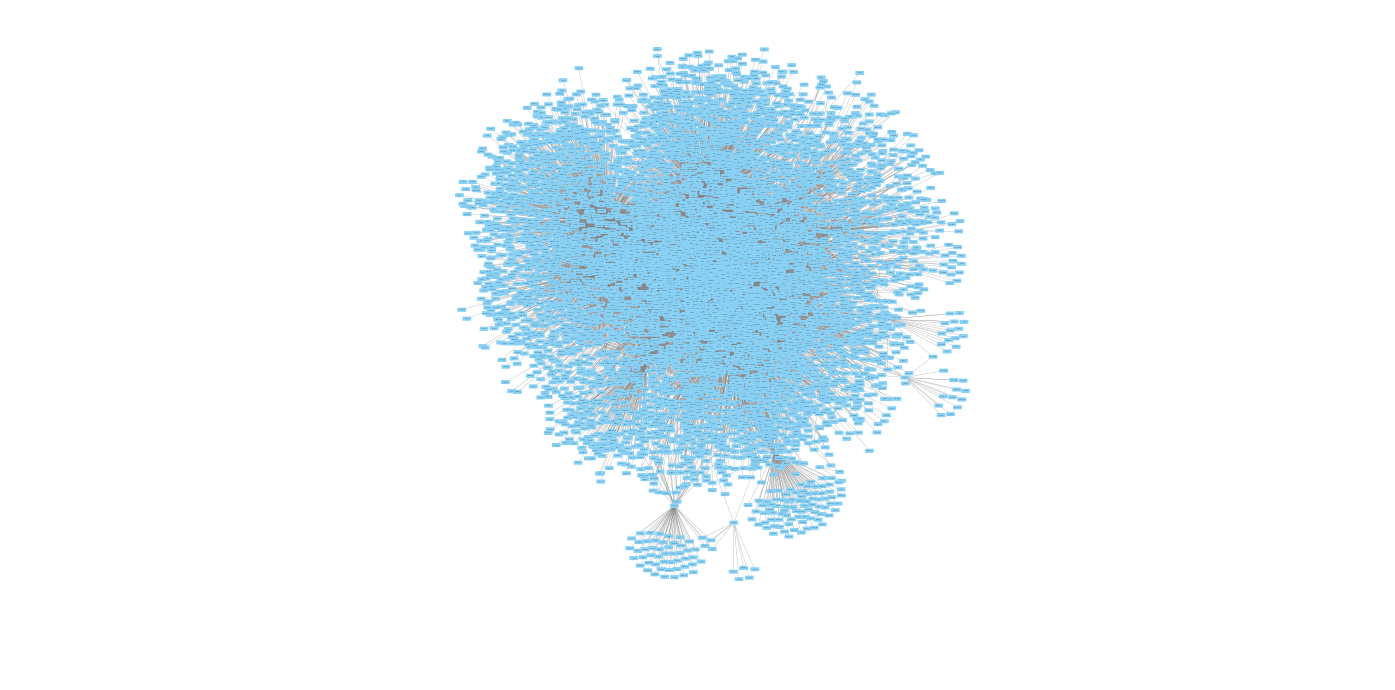
\includegraphics{g.graphml.png}
\caption{Disease interactome graph.}
\end{figure}

\hypertarget{first-20-highest-ranking-genes-for-betweenness}{%
\subsubsection{First 20 highest ranking genes for
betweenness}\label{first-20-highest-ranking-genes-for-betweenness}}

\begin{table}[H]
\centering
\begin{tabular}[t]{l|r|r|r|r|r}
\hline
X & nodes\_degree & nodes\_betweenness\_centrality & eigen\_vector\_centrality & closeness\_centrality & betweennes\_degree\_ratio\\
\hline
MYC & 1956 & 0.3520452 & 0.4743706 & 0.4927457 & 0.0001800\\
\hline
KRAS & 1593 & 0.2766164 & 0.3086325 & 0.4477919 & 0.0001736\\
\hline
TP53 & 1328 & 0.2274370 & 0.2893261 & 0.4759286 & 0.0001713\\
\hline
CTNNB1 & 708 & 0.0858398 & 0.1839057 & 0.4512143 & 0.0001212\\
\hline
CDH1 & 657 & 0.0823632 & 0.1306841 & 0.4133892 & 0.0001254\\
\hline
HRAS & 633 & 0.0791818 & 0.1184252 & 0.4287654 & 0.0001251\\
\hline
IKBKG & 393 & 0.0657733 & 0.0638395 & 0.4120947 & 0.0001674\\
\hline
MAPK1 & 330 & 0.0466317 & 0.0734102 & 0.4473479 & 0.0001413\\
\hline
STAT3 & 294 & 0.0399930 & 0.0567409 & 0.3977208 & 0.0001360\\
\hline
PML & 276 & 0.0359068 & 0.0755400 & 0.4489056 & 0.0001301\\
\hline
TK1 & 204 & 0.0351768 & 0.0354053 & 0.3988005 & 0.0001724\\
\hline
TNF & 301 & 0.0304197 & 0.0533508 & 0.3549275 & 0.0001011\\
\hline
RB1 & 259 & 0.0275146 & 0.0640836 & 0.4109954 & 0.0001062\\
\hline
MAPK3 & 243 & 0.0274794 & 0.0555375 & 0.4181228 & 0.0001131\\
\hline
CCNDBP1 & 131 & 0.0270992 & 0.0078218 & 0.3352261 & 0.0002069\\
\hline
PRDX1 & 217 & 0.0230300 & 0.0479814 & 0.3914121 & 0.0001061\\
\hline
TGFB1 & 258 & 0.0228321 & 0.0554258 & 0.3541912 & 0.0000885\\
\hline
CCND1 & 224 & 0.0194292 & 0.0581923 & 0.3814153 & 0.0000867\\
\hline
GSTP1 & 147 & 0.0190903 & 0.0293582 & 0.3828717 & 0.0001299\\
\hline
BCL2L1 & 181 & 0.0187980 & 0.0459919 & 0.4063425 & 0.0001039\\
\hline
CXCL9 & 74 & 0.0165921 & 0.0010691 & 0.3052871 & 0.0002242\\
\hline
MET & 127 & 0.0158673 & 0.0429730 & 0.4194834 & 0.0001249\\
\hline
GJB1 & 76 & 0.0151805 & 0.0059988 & 0.3325962 & 0.0001997\\
\hline
BCL2 & 113 & 0.0133933 & 0.0417643 & 0.4377685 & 0.0001185\\
\hline
SOCS1 & 148 & 0.0126367 & 0.0336162 & 0.3737870 & 0.0000854\\
\hline
ENO2 & 108 & 0.0124763 & 0.0129452 & 0.3322988 & 0.0001155\\
\hline
FAS & 111 & 0.0123463 & 0.0193346 & 0.3585131 & 0.0001112\\
\hline
SPP1 & 92 & 0.0119589 & 0.0099339 & 0.3318624 & 0.0001300\\
\hline
TSC22D1 & 93 & 0.0095640 & 0.0160543 & 0.3586352 & 0.0001028\\
\hline
TNFRSF10B & 74 & 0.0090746 & 0.0086328 & 0.3326663 & 0.0001226\\
\hline
\end{tabular}
\end{table}

\end{document}
